\begin{figure*}[hb!]
    \label{fig:epitope_graph}
    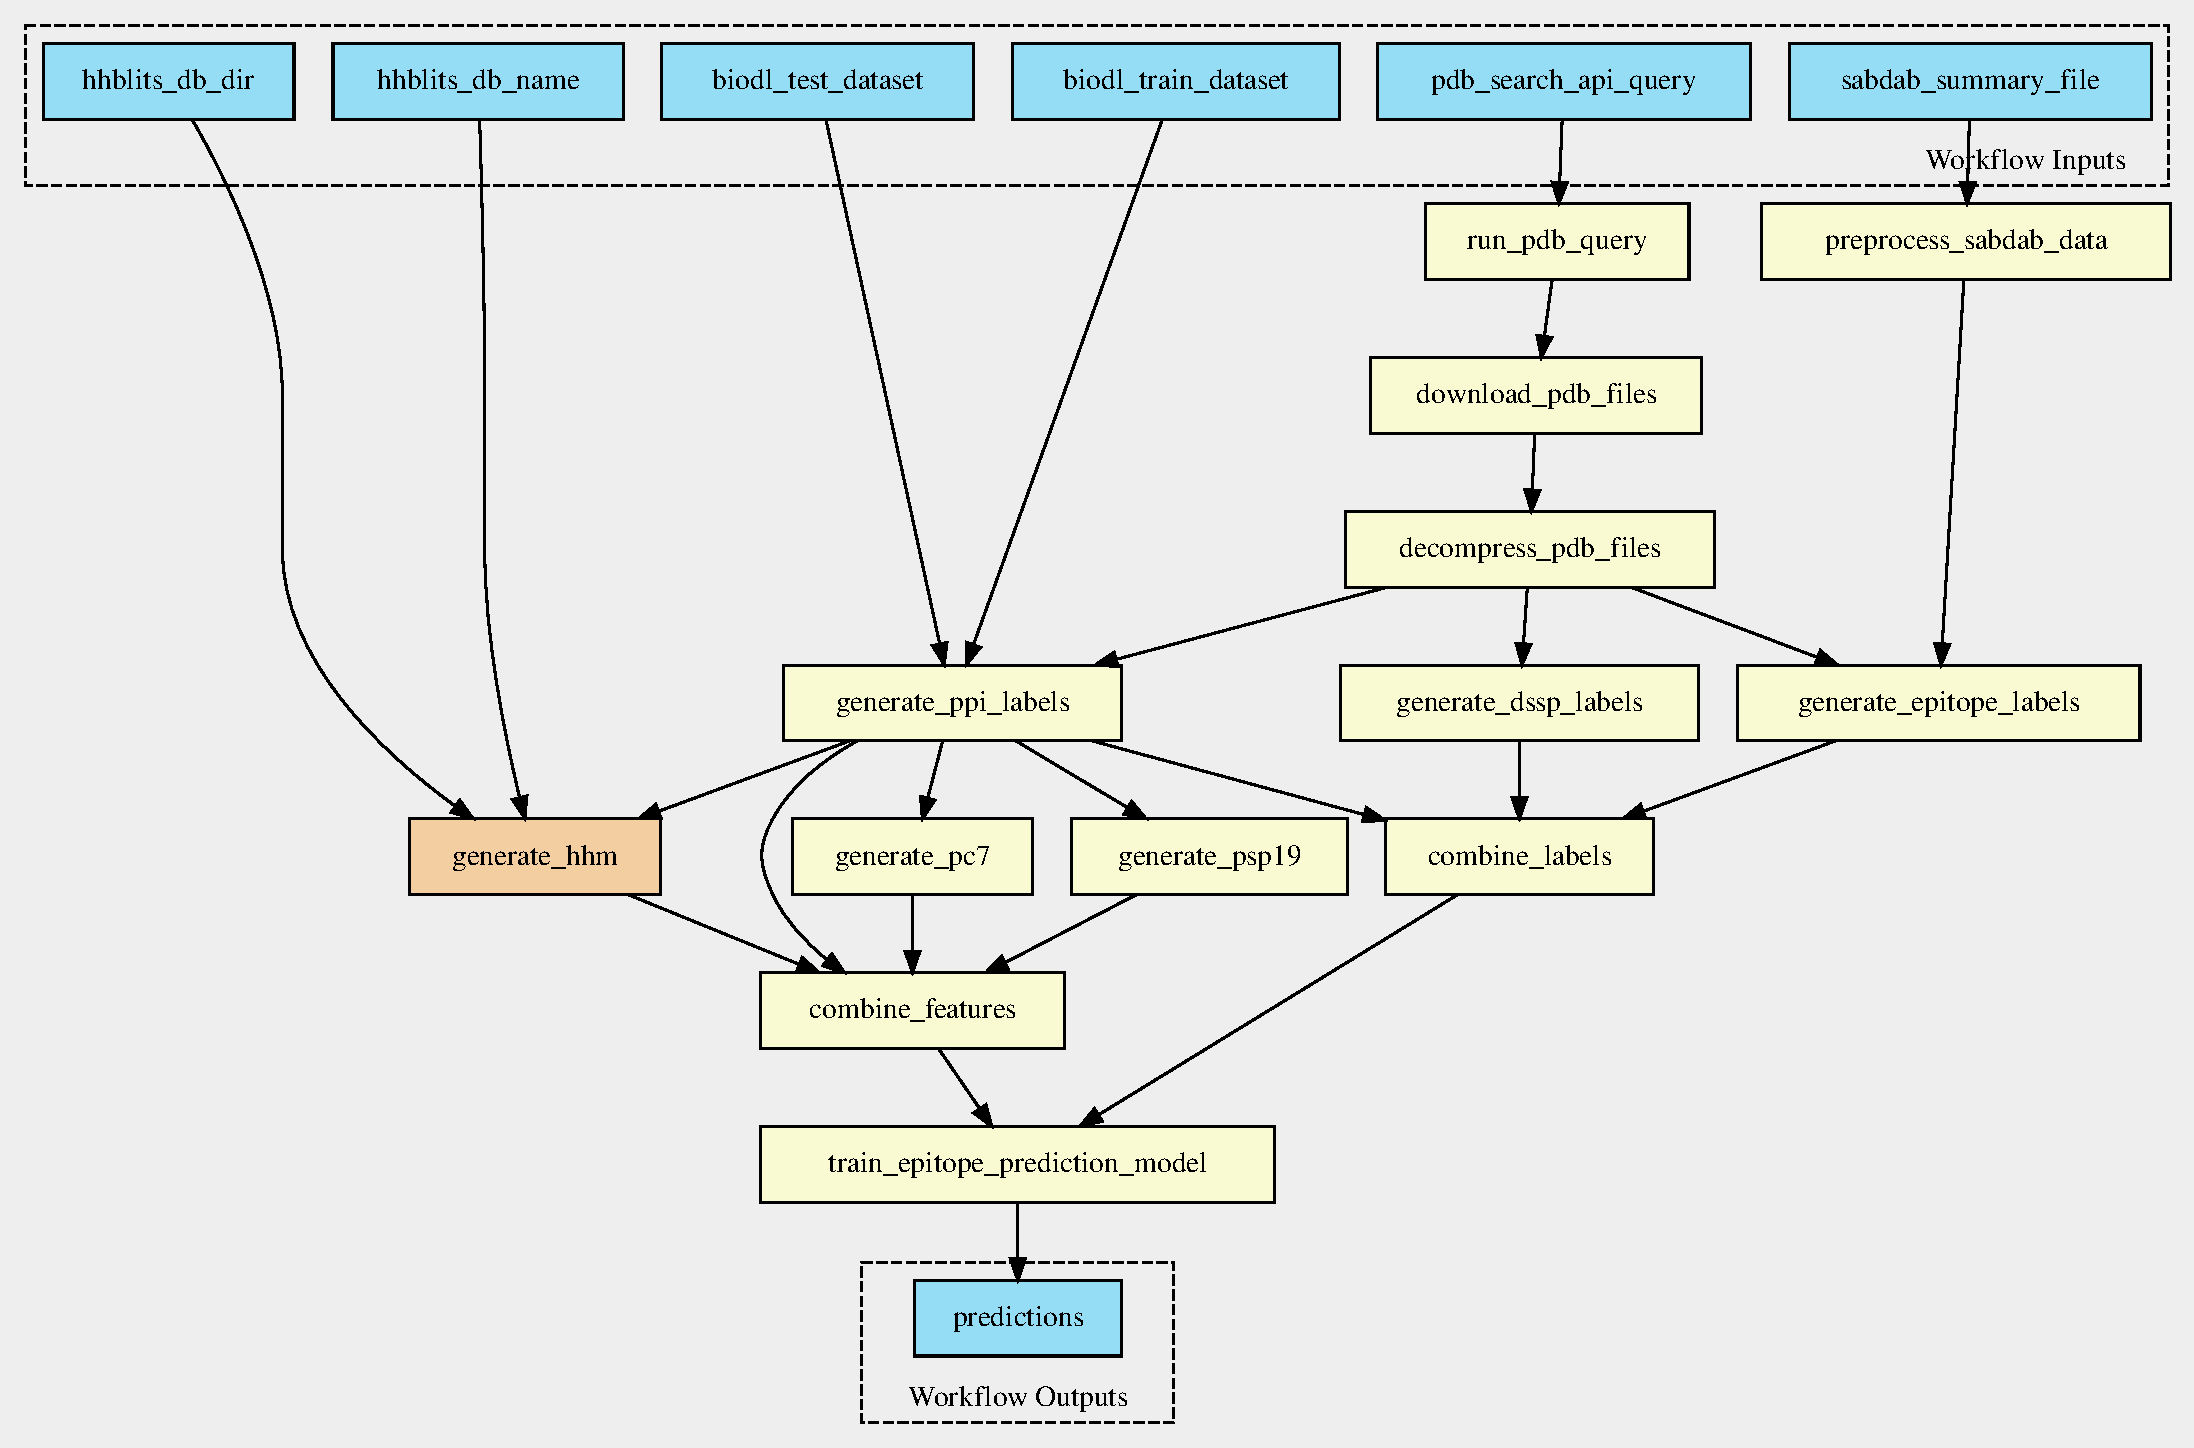
\includegraphics[width=1\linewidth]{taxonomy/workflow.pdf}
    \caption{CWL implementation of the workflow we used as an example. Based on data retrieved from multiple FAIR and non-FAIR resources, the workflow computes a set of input features and labels. These are subsequently used to train a deep learning model which predicts the amino acids in a protein which are likely to be \emph{epitopes}, i.e. binding sites for antibodies. Based on our experience, this workflow is exemplary for many problems which commonly arise when reproducing computational results.
    Nodes represent the steps, edges signify data flow between the steps. Yellow nodes indicate steps which run \emph{CommandLineTools}, orange nodes represent steps which control nested \emph{Workflows}, blue nodes signify workflow input and output parameters. }
    \label{fig:wf}
\end{figure*}